\documentclass[11pt,a4paper]{article}
\usepackage[utf8]{inputenc}
\usepackage[T1]{fontenc}
\usepackage[margin=1in]{geometry}
\usepackage{graphicx}
\usepackage{hyperref}
\usepackage{xcolor}
\usepackage{float}
\usepackage{listings}
\usepackage{upquote}
\usepackage{amsmath}

% Code listing style
\lstset{
    basicstyle=\ttfamily\small,
    breaklines=true,
    breakatwhitespace=false,
    frame=single,
    numbers=left,
    numberstyle=\tiny,
    backgroundcolor=\color{gray!10},
    keywordstyle=\color{blue},
    commentstyle=\color{green!50!black},
    stringstyle=\color{red},
    showstringspaces=false
}

\title{\textbf{Practice 3 - Visual Servoing}}
\author{
    Robotics and Cyber-Physical Systems \\
    School of Sciences and Engineering \\
    Tecnol\'ogico de Monterrey
}
\date{}

\begin{document}

\maketitle

\section*{Introduction}

This practice introduces visual servoing—the technique of using camera feedback to control robot motion. You will learn how to process camera images, detect objects using color segmentation, compute visual error signals, and implement closed-loop control that moves the robot to center objects in its field of view.

The practice is structured in five progressive parts: first you'll add manual control to the boilerplate, then display camera feeds (RGB and depth), create a color mask visualization, implement proportional visual servoing with manual override, and finally integrate depth measurements. By the end, you'll have a complete system that tracks colored objects while allowing operator intervention and displaying real-time distance information.

Each part builds on the previous one, developing a complete understanding of vision-based robot control through the \texttt{stretch\_toolkit} interface.

\subsection*{Before You Begin}

If you previously cloned this repository, update it to the latest version to ensure you have all the necessary files and recent improvements. \textbf{Important:} The update command below will overwrite any local changes you've made. If you have files you want to keep (such as solutions to previous activities), make a backup copy outside the repository folder before proceeding.

To update your repository:

\begin{lstlisting}[language=bash]
git pull
git fetch origin
git reset --hard origin/main
\end{lstlisting}

If dependencies were updated, synchronize your environment:

\begin{lstlisting}[language=bash]
uv sync
\end{lstlisting}

\newpage

\section*{Part 1 - Manual Control Foundation}

Before implementing visual servoing, you need a working control system. In this part, you'll add manual control to the boilerplate so you can position the robot using a gamepad or keyboard.

\subsection*{Objective}

Add teleoperation capabilities to \texttt{stretch\_boilerplate.py}, enabling manual control of the robot's head and base. This provides the foundation for later parts where you'll blend autonomous visual servoing with operator override.

\subsection*{Task}

Copy \texttt{stretch\_boilerplate.py} to a new file called \texttt{p3\_1\_manual.py}. 

In the boilerplate, the main loop currently has a placeholder for your logic:

\begin{lstlisting}[language=Python]
while True:
    # --- Loop setup ---
    t = controller.get_time()
    velocities = {}

    # --- Your logic here ---

    # --- Send commands ---
    controller.set_velocities(velocities)
    cv2.waitKey(1)
    time.sleep(1 / 30)  # 30 Hz
\end{lstlisting}

The \texttt{teleop} object provides a method \texttt{get\_normalized\_velocities()} that returns a dictionary of joint velocities based on the current state of your gamepad or keyboard. Retrieve these velocities and assign them to the \texttt{velocities} variable.

After your changes, the loop should look like this:

\begin{lstlisting}[language=Python]
while True:
    # --- Loop setup ---
    t = controller.get_time()
    velocities = {}

    # --- Your logic here ---
    velocities = teleop.get_normalized_velocities()

    # --- Send commands ---
    controller.set_velocities(velocities)
    cv2.waitKey(1)
    time.sleep(1 / 30)  # 30 Hz
\end{lstlisting}

\subsection*{Expected Result}

Run your script and verify that you can manually control the robot:

\begin{lstlisting}[language=bash]
uv run p3_1_manual.py
\end{lstlisting}

You should be able to:
\begin{itemize}
    \item Drive the base forward/backward and rotate left/right
    \item Pan and tilt the head camera
    \item Extend and retract the arm
\end{itemize}

\textbf{Note:} The boilerplate already imports \texttt{teleop} and sets up the control loop structure. Your task is to connect the teleop input to the controller output with a single line of code.

\newpage

\section*{Part 2 - Camera Feed Display}

Visual servoing requires camera input. In this part, you'll display both RGB and depth camera feeds from the robot's head camera, maintaining manual control from Part 1.

\subsection*{Objective}

Extend \texttt{p3\_1\_manual.py} to display live camera feeds in separate windows. This allows you to see what the robot sees while controlling it manually—essential for understanding the visual feedback used in later parts.

\subsection*{Task}

Copy \texttt{p3\_1\_manual.py} to a new file called \texttt{p3\_2\_cameras.py}.

The boilerplate already imports \texttt{HEAD\_RGB\_CAMERA} and \texttt{HEAD\_DEPTH\_CAMERA}. These camera objects provide a \texttt{get\_frame()} method that returns the current image as a NumPy array.

Add code to:
\begin{enumerate}
    \item Retrieve the RGB frame from \texttt{HEAD\_RGB\_CAMERA}
    \item Retrieve the depth frame from \texttt{HEAD\_DEPTH\_CAMERA}
    \item Display the RGB frame in a window called "RGB Camera"
    \item Display the depth frame in a window called "Depth Camera"
\end{enumerate}

Use OpenCV's \texttt{cv2.imshow(window\_name, image)} function to display images. Place this code inside the main loop, before or after sending velocities—either works.

\subsection*{Expected Result}

Run your script:

\begin{lstlisting}[language=bash]
uv run p3_2_cameras.py
\end{lstlisting}

You should see two windows open:
\begin{itemize}
    \item \textbf{RGB Camera}: showing the color view from the robot's head
    \item \textbf{Depth Camera}: showing depth information (closer objects appear brighter)
\end{itemize}

Manual control should still work—you can pan/tilt the head and see the camera views update in real time.

\begin{figure}[H]
    \centering
    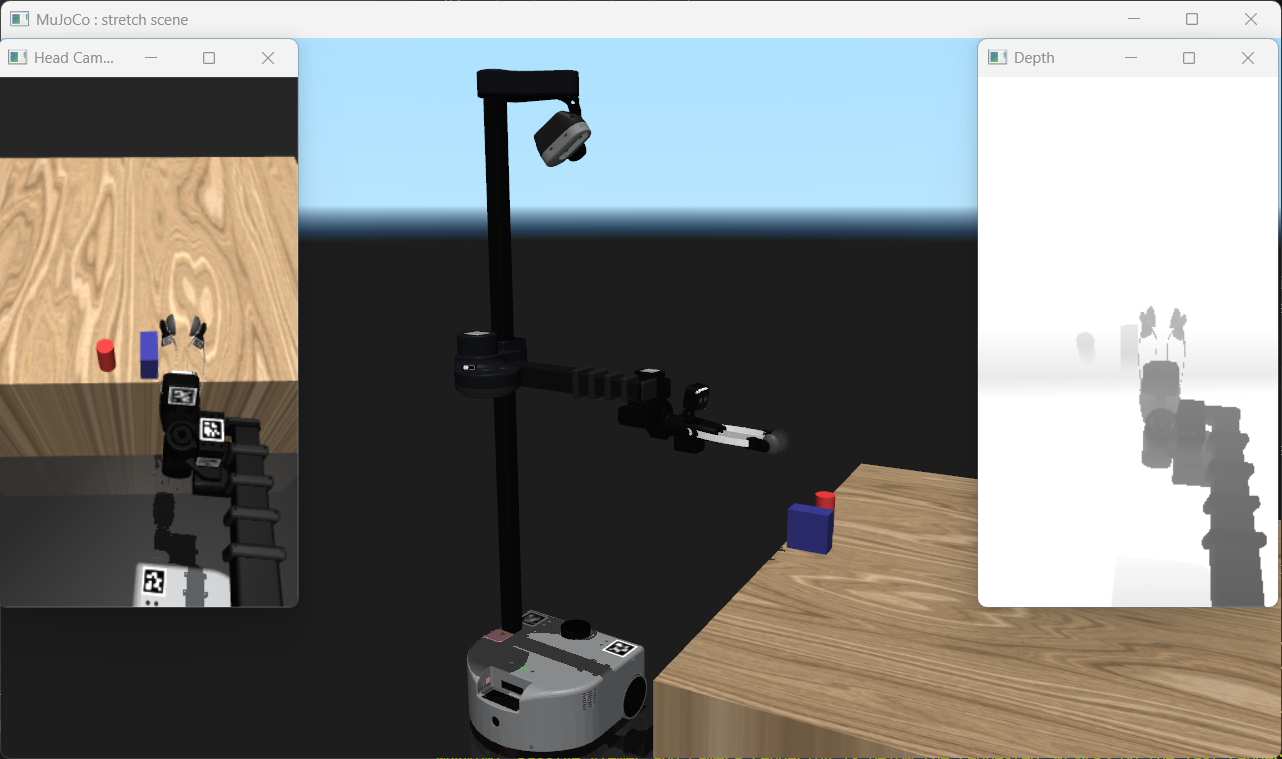
\includegraphics[width=0.8\textwidth]{p3_2_cameras.png}
    \caption{RGB and depth camera windows displaying simultaneously}
    \label{fig:p3_2_cameras}
\end{figure}

\newpage

\section*{Part 3 - Color Detection Mask}

To track colored objects, you need to segment the image based on color. In this part, you'll create a binary mask that isolates blue objects in the camera view.

\subsection*{Objective}

Add color-based segmentation to visualize which pixels in the RGB image match your target color (blue). This mask will be used in Part 4 to locate the object's position.

\subsection*{Task}

Copy \texttt{p3\_2\_cameras.py} to a new file called \texttt{p3\_3\_mask.py}.

Color detection in computer vision typically uses the HSV (Hue, Saturation, Value) color space rather than RGB. HSV separates color information (hue) from brightness (value), making it more robust for color-based segmentation.

Add code to:
\begin{enumerate}
    \item Convert the RGB frame to HSV using \texttt{cv2.cvtColor(rgb\_frame, cv2.COLOR\_BGR2HSV)}
    \item Define lower and upper HSV bounds for blue. For example:
    \begin{lstlisting}[language=Python]
lower_blue = np.array([110, 100, 100])
upper_blue = np.array([130, 255, 255])
    \end{lstlisting}
    \item Create a binary mask using \texttt{cv2.inRange(hsv\_frame, lower\_blue, upper\_blue)}
    \item Display the mask in a third window called "Blue Mask"
\end{enumerate}

The \texttt{cv2.inRange()} function returns a binary image where pixels within the HSV range are white (255) and all others are black (0).

\textbf{Note on HSV values:} Hue ranges from 0-179 in OpenCV (not 0-360). Blue is typically around 110-130. Saturation and Value range from 0-255. Adjust these ranges if your blue object isn't detected properly.

\subsection*{Expected Result}

Run your script:

\begin{lstlisting}[language=bash]
uv run p3_3_mask.py
\end{lstlisting}

You should see three windows:
\begin{itemize}
    \item \textbf{RGB Camera}: the original color view
    \item \textbf{Depth Camera}: depth information
    \item \textbf{Blue Mask}: binary mask showing detected blue regions in white
\end{itemize}

Point the camera at a blue object—it should appear as a white blob in the mask window. Non-blue areas should be black.

\begin{figure}[H]
    \centering
    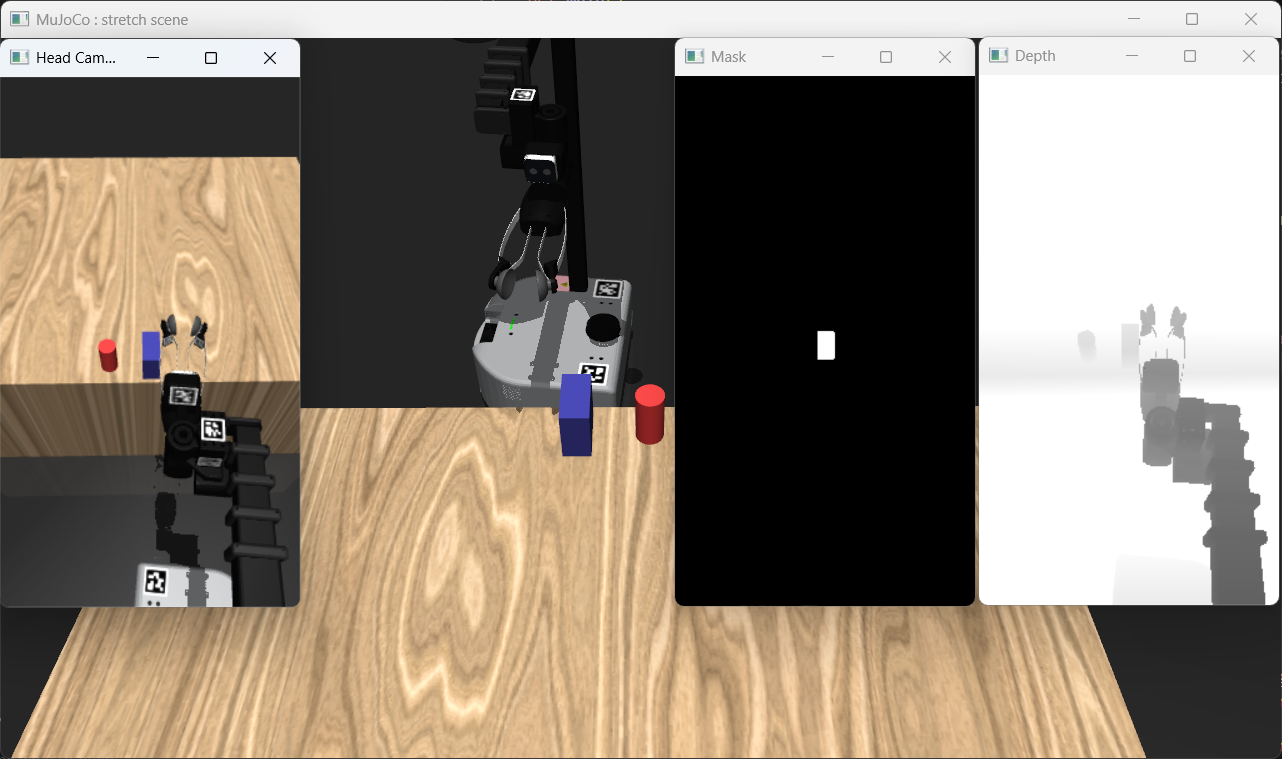
\includegraphics[width=0.8\textwidth]{p3_3_mask.png}
    \caption{Three windows showing RGB camera, depth camera, and blue object mask}
    \label{fig:p3_3_mask}
\end{figure}

\newpage

\section*{Part 4 - Visual Servoing with Manual Override}

Now you'll implement closed-loop visual servoing: the robot will automatically move its head to center the blue object in the camera view, while still allowing manual override.

\subsection*{Objective}

Use the binary mask from Part 3 to compute the object's position, calculate control commands to center it, and blend autonomous servoing with manual control using proportional blending.

\subsection*{Task}

Copy \texttt{p3\_3\_mask.py} to a new file called \texttt{p3\_4\_servo.py}.

Visual servoing requires three steps: detect the object, compute the error, and apply proportional control.

\subsubsection*{Step 1: Find the Object's Centroid}

Use \texttt{cv2.findContours()} to find contours (connected white regions) in the binary mask. If contours are found, select the largest one and compute its centroid using \texttt{cv2.moments()}.

The centroid gives you the (x, y) pixel coordinates of the object's center. Image coordinates are typically (0,0) at the top-left corner.

\begin{lstlisting}[language=Python]
contours, _ = cv2.findContours(mask, cv2.RETR_EXTERNAL, 
                                cv2.CHAIN_APPROX_SIMPLE)
if contours:
    largest_contour = max(contours, key=cv2.contourArea)
    M = cv2.moments(largest_contour)
    if M["m00"] > 0:
        cx = int(M["m10"] / M["m00"])
        cy = int(M["m01"] / M["m00"])
\end{lstlisting}

\subsubsection*{Step 2: Calculate Visual Error}

Compute the error between the object's centroid and the image center. Get the image dimensions using \texttt{rgb\_frame.shape}, then calculate:

\begin{lstlisting}[language=Python]
height, width = rgb_frame.shape[:2]
error_x = cx - width // 2
error_y = cy - height // 2
\end{lstlisting}

\subsubsection*{Step 3: Proportional Control}

Apply proportional control to generate servo velocities. The head pan should respond to horizontal error (error\_x) and head tilt to vertical error (error\_y). Use a gain constant (e.g., $K_p = 0.5$) to scale the error to appropriate velocity:

\begin{lstlisting}[language=Python]
Kp = 0.5
servo_velocities = {
    "head_pan": -Kp * error_x / width,
    "head_tilt": Kp * error_y / height
}
\end{lstlisting}

Note the negative sign on pan—when the object is to the right (positive error\_x), the robot should pan right (positive velocity), but due to coordinate conventions this requires negation.

\subsubsection*{Step 4: Blend with Manual Control}

Don't replace the teleop velocities directly—blend them using \texttt{merge\_proportional()}. This function from \texttt{stretch\_toolkit} combines manual and autonomous commands, giving priority to manual control when the operator provides input:

\begin{lstlisting}[language=Python]
teleop_velocities = teleop.get_normalized_velocities()
velocities = merge_proportional(teleop_velocities, servo_velocities)
\end{lstlisting}

\subsection*{Expected Result}

Run your script:

\begin{lstlisting}[language=bash]
uv run p3_4_servo.py
\end{lstlisting}

The robot should automatically pan and tilt its head to keep the blue object centered in the camera view. You can still manually control the robot—when you move the head, the autonomous servoing remains active but yields to your commands.

Try these tests:
\begin{itemize}
    \item Let the robot track the object autonomously
    \item Move the object around—the robot should follow it
    \item Manually override by moving the head—control should be smooth
    \item Release the manual controls—servoing should resume
\end{itemize}

\begin{figure}[H]
    \centering
    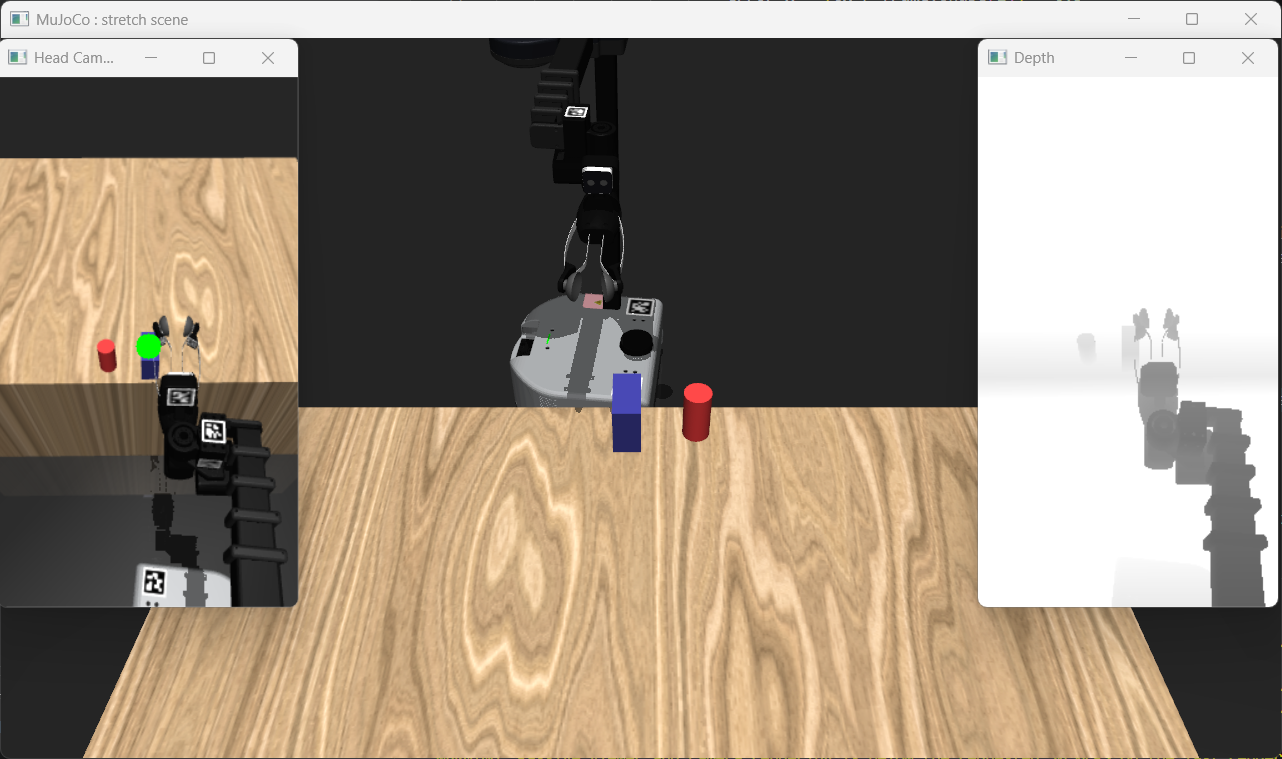
\includegraphics[width=0.8\textwidth]{p3_4_servo.png}
    \caption{Robot performing visual servoing with object centered in view}
    \label{fig:p3_4_servo}
\end{figure}

\subsection*{Optional: Distance Measurement}

Once you have the object's centroid coordinates, you can measure the distance to it using the depth camera. The \texttt{HEAD\_CAMERA} object provides a \texttt{get\_depth(x, y)} method that returns the distance in meters to the pixel at coordinates (x, y).

\begin{lstlisting}[language=Python]
distance = HEAD_CAMERA.get_depth(cx, cy)
print(f"Distance to object: {distance:.2f}m")
\end{lstlisting}

You can also display the distance on the RGB frame using \texttt{cv2.putText()}:

\begin{lstlisting}[language=Python]
cv2.putText(rgb_frame, f"Distance: {distance:.2f}m", 
            (10, 30), cv2.FONT_HERSHEY_SIMPLEX, 
            1, (0, 255, 0), 2)
\end{lstlisting}

This provides real-time feedback about how far away the tracked object is, which is useful for approach behaviors or obstacle avoidance.

\newpage

\section*{Deliverable}

Submit a screen recording with voiceover demonstrating your completed visual servoing system from Part 4.

Your video should show:
\begin{itemize}
    \item All three windows visible (RGB Camera, Depth Camera, Blue Mask)
    \item The robot autonomously tracking a blue object
    \item Manual override working smoothly with autonomous control
    \item Optional: distance measurement displayed
\end{itemize}

In your voiceover, briefly explain how the system works—covering HSV segmentation, proportional control, and the \texttt{merge\_proportional()} blending function.

\end{document}
